\documentclass[answers,12pt,addpoints]{exam}
\usepackage{amsmath}
\usepackage{amsfonts}
\usepackage{amssymb}
\usepackage{mathrsfs}
\usepackage{dsfont}
\usepackage{cancel}
\usepackage{graphicx}
\usepackage{import}

\import{C:/Users/prana/OneDrive/Desktop/MathNotes}{style.tex}

% Header
\newcommand{\name}{Pranav Tikkawar}
\newcommand{\course}{01:640:423}
\newcommand{\assignment}{Homework 3}
\author{\name}
\title{\course \ - \assignment}

\begin{document}
\maketitle
\begin{questions}

\question Section 2.1 Problem 5\\
(The hammer blow) Let $\phi(x) \equiv 0$ and $\psi(x) = 1$ for $|x| < a$ and $\psi(x) = 0$ for $|x| \geq a$. Sketch the string profile (u vs x) at each of the sucesses instances: $t = a/2c, a/c, 3a/2c, 2a/c, \text{ and } 5a/c$. Hint:[ Calculate
$$ u(x,t) = \frac{1}{2c} \int_{x-ct}^{x+ct} \psi(s) ds = \frac{1}{2c} \text{ length of } (x-ct,x+ct) \cap (-a,a)$$
Then $u(x, a/2c) = (1/2c)${ length of $(x-ct,x+ct) \cap (-a,a)$} This takes on different values for $|x| < a/2$ for $a/2 < x < 3a/2$ and for $x > 3a/2$. Continue this for the other times.]
\textbf{Solution:}\\
\begin{align*}
    u_{tt} &= c^2 u_{xx} \\
    u(x,0) &= 0 \\
    u_t(x,0) &= \begin{cases}
    0 & \text{if } |x| \geq a \\
    1 & \text{if } |x| < a
    \end{cases}
\end{align*}
We can use D'Alemberts formula to solve this problem. We have
$$ u(x,t) = \frac{1}{2} \left[ \phi(x+ct) + \phi(x-ct) \right] + \frac{1}{2c} \int_{x-ct}^{x+ct} \psi(s) ds $$
Since $\phi(x) = 0$, we have
$$ u(x,t) = \frac{1}{2c} \int_{x-ct}^{x+ct} \psi(s) ds$$
Clealry since $\psi(x) = 1$ for $|x| < a$ We only need to consider:
$$ u(x,t) = \frac{1}{2c} \int_{x-ct}^{x+ct} ds = \frac{1}{2c} \text{ length of } (x-ct,x+ct) \cap (-a,a)$$

Since we know that the wave function is even, ie $u(x,t) = u(-x,t)$, we only need to consider the case when $x > 0$ and for any interval that a function of $x$ will need to have a negative $x$ for the corresponding interval.\\

\textbf{Case 1: $t = a/2c$}\\
We can see that $x \pm a/2$ becomes the boundary of the interval. \\
We can consider the following cases:
\begin{itemize}
    \item $ x \in (-a/2, a/2)$
    \item $ x \in (a/2, 3a/2)$
    \item $ x \in (3a/2, \infty)$
\end{itemize}
\textbf{Subcase 1: $x \in (-a/2, a/2)$}\\
$$(x-a/2, x+a/2) \cap (-a,a) = (x-a/2, x+a/2)$$
$$u(x,a/2c) = \frac{1}{2c} \int_{x-a/2}^{x+a/2} ds = \frac{a}{2c}$$

\textbf{Subcase 2: $x \in (a/2, 3a/2)$}\\
$$(x-a/2, x+a/2) \cap (-a,a) = (x-a/2, a)$$
$$u(x,a/2c) = \frac{1}{2c} \int_{x-a/2}^{a} ds = \frac{3a-2x}{4c}$$

\textbf{Subcase 3: $x \in (3a/2, \infty)$}\\
$$(x-a/2, x+a/2) \cap (-a,a) = \emptyset$$
$$u(x,a/2c) = \frac{1}{2c} \int_{a}^{a} ds = 0$$
\textbf{Plotting the graph}\\
\begin{center}
    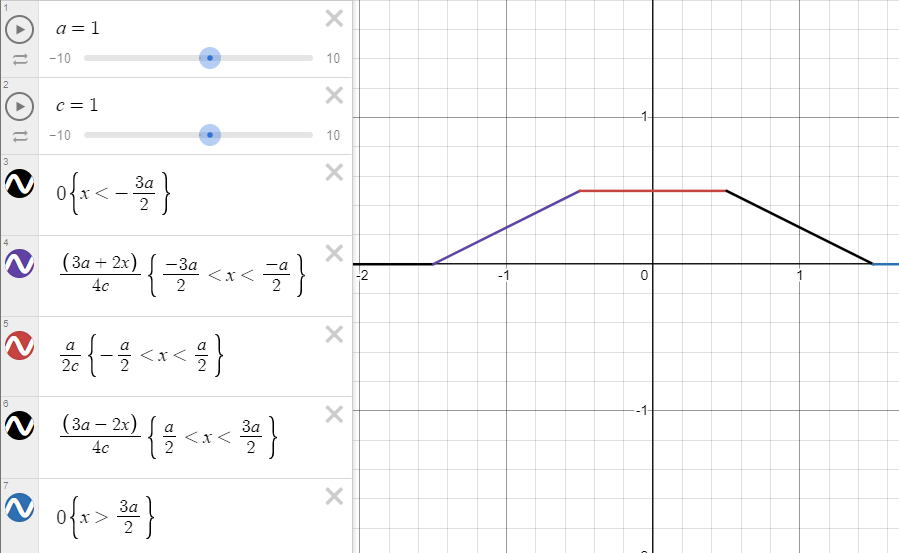
\includegraphics[scale = 0.5]{HW3IMG/11.png}
\end{center}



\textbf{Case 2: $t = a/c$}\\
We can see that $x \pm a$ becomes the boundary of the interval. \\
We can consider the following cases:
\begin{itemize}
    \item $ x \in (0, 2a)$
    \item $ x \in (2a, \infty)$
\end{itemize}
\textbf{Subcase 1: $x \in (0, 2a)$}\\
$$(x-a, x+a) \cap (-a,a) = (x-a, a)$$
$$u(x,a/c) = \frac{1}{2c} \int_{x-a}^{a} ds = \frac{2a-x}{2c}$$

\textbf{Subcase 2: $x \in (2a, \infty)$}\\
$$(x-a, x+a) \cap (-a,a) = \emptyset$$
$$u(x,a/c) = \frac{1}{2c} \int_{a}^{a} ds = 0$$

\textbf{Plotting the graph}\\
\begin{center}
    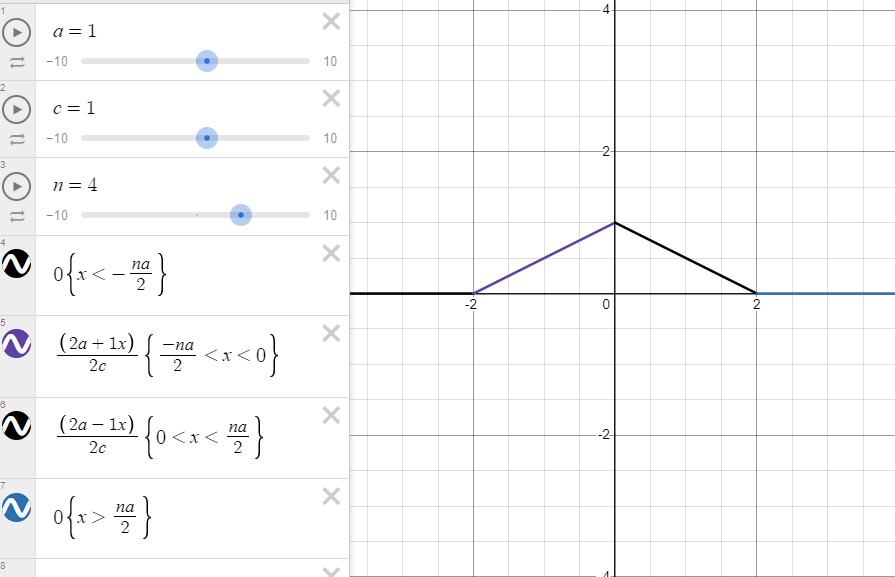
\includegraphics[scale = 0.5]{HW3IMG/12.png}
\end{center}

\textbf{Case 3: $t = 3a/2c$}\\
We can see that $x \pm 3a/2$ becomes the boundary of the interval. \\
We can consider the following cases:
\begin{itemize}
    \item $ x \in (-a/2, a/2)$
    \item $ x \in (a/2, 5a/2)$
    \item $ x \in (5a/2, \infty)$
\end{itemize}
\textbf{Subcase 1: $x \in (-a/2, a/2)$}\\
$$(x-3a/2, x+3a/2) \cap (-a,a) = (-a,a)$$
$$u(x,3a/2c) = \frac{1}{2c} \int_{-a}^{a} ds = \frac{a}{c}$$

\textbf{Subcase 2: $x \in (a/2, 5a/2)$}\\
$$(x-3a/2, x+3a/2) \cap (-a,a) = (x-3a/2, a)$$
$$u(x,3a/2c) = \frac{1}{2c} \int_{x-3a/2}^{a} ds = \frac{1}{2c}(\frac{5a}{2}-x)$$

\textbf{Subcase 3: $x \in (5a/2, \infty)$}\\
$$(x-3a/2, x+3a/2) \cap (-a,a) = \emptyset$$
$$u(x,3a/2c) = \frac{1}{2c} \int_{a}^{a} ds = 0$$

\textbf{Plotting the graph}\\

\begin{center}
    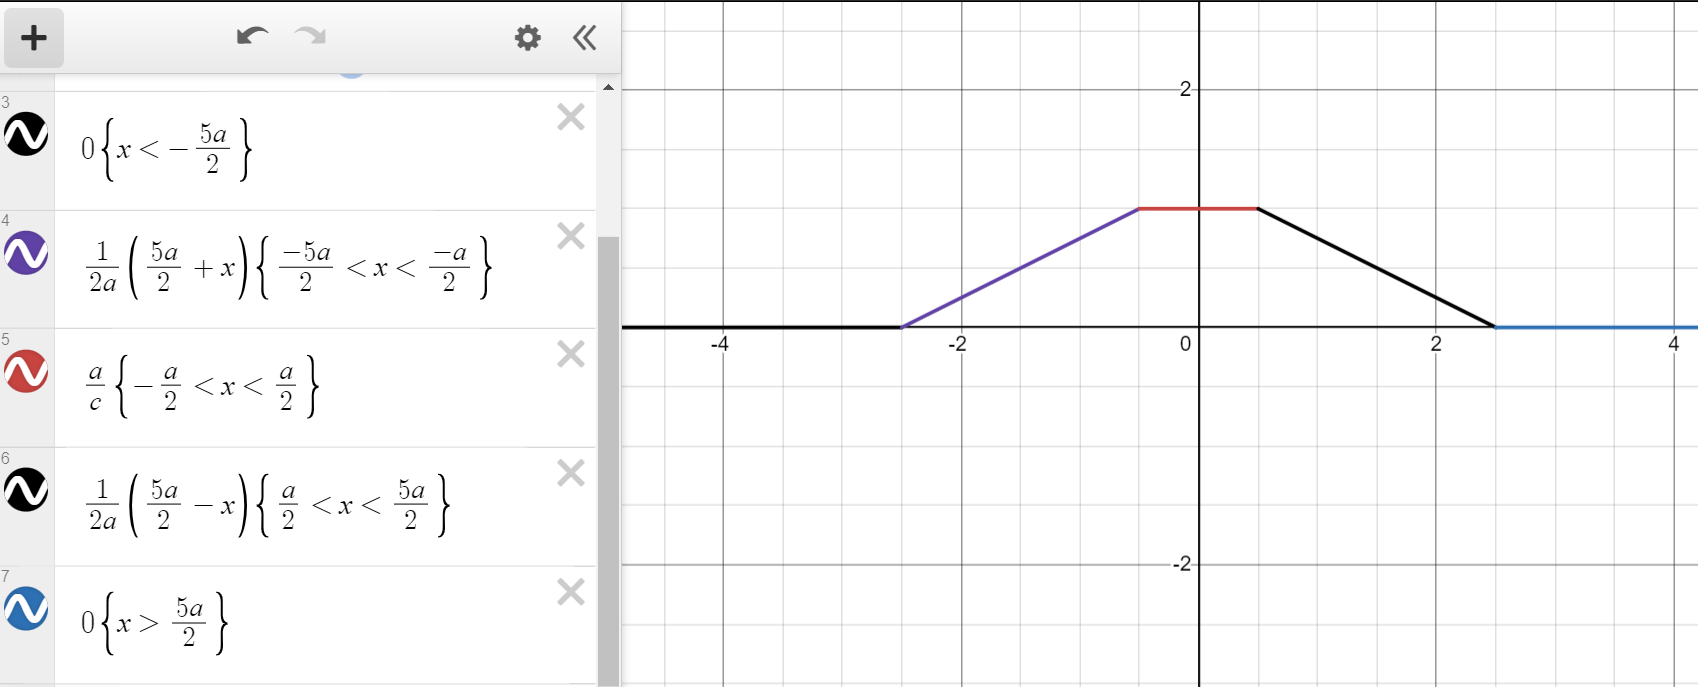
\includegraphics[scale = 0.5]{HW3IMG/13.png}
\end{center}


\textbf{Case 4: $t = 2a/c$}\\
We can see that $x \pm 2a$ becomes the boundary of the interval. \\
We can consider the following cases:
\begin{itemize}
    \item $ x \in (-a, a)$
    \item $ x \in (a, 3a)$
    \item $ x \in (3a, \infty)$
\end{itemize}
\textbf{Subcase 1: $x \in (-a, a)$}\\
$$(x-2a, x+2a) \cap (-a,a) = (-a,a)$$
$$u(x,2a/c) = \frac{1}{2c} \int_{-a}^{a} ds = \frac{a}{c}$$

\textbf{Subcase 2: $x \in (a, 3a)$}\\
$$(x-2a, x+2a) \cap (-a,a) = (x-2a, a)$$
$$u(x,2a/c) = \frac{1}{2c} \int_{x-2a}^{a} ds = \frac{1}{2c}({3a}-x)$$

\textbf{Subcase 3: $x \in (3a, \infty)$}\\
$$(x-2a, x+2a) \cap (-a,a) = \emptyset$$
$$u(x,2a/c) = \frac{1}{2c} \int_{a}^{a} ds = 0$$

\textbf{Plotting the graph}\\

\begin{center}
    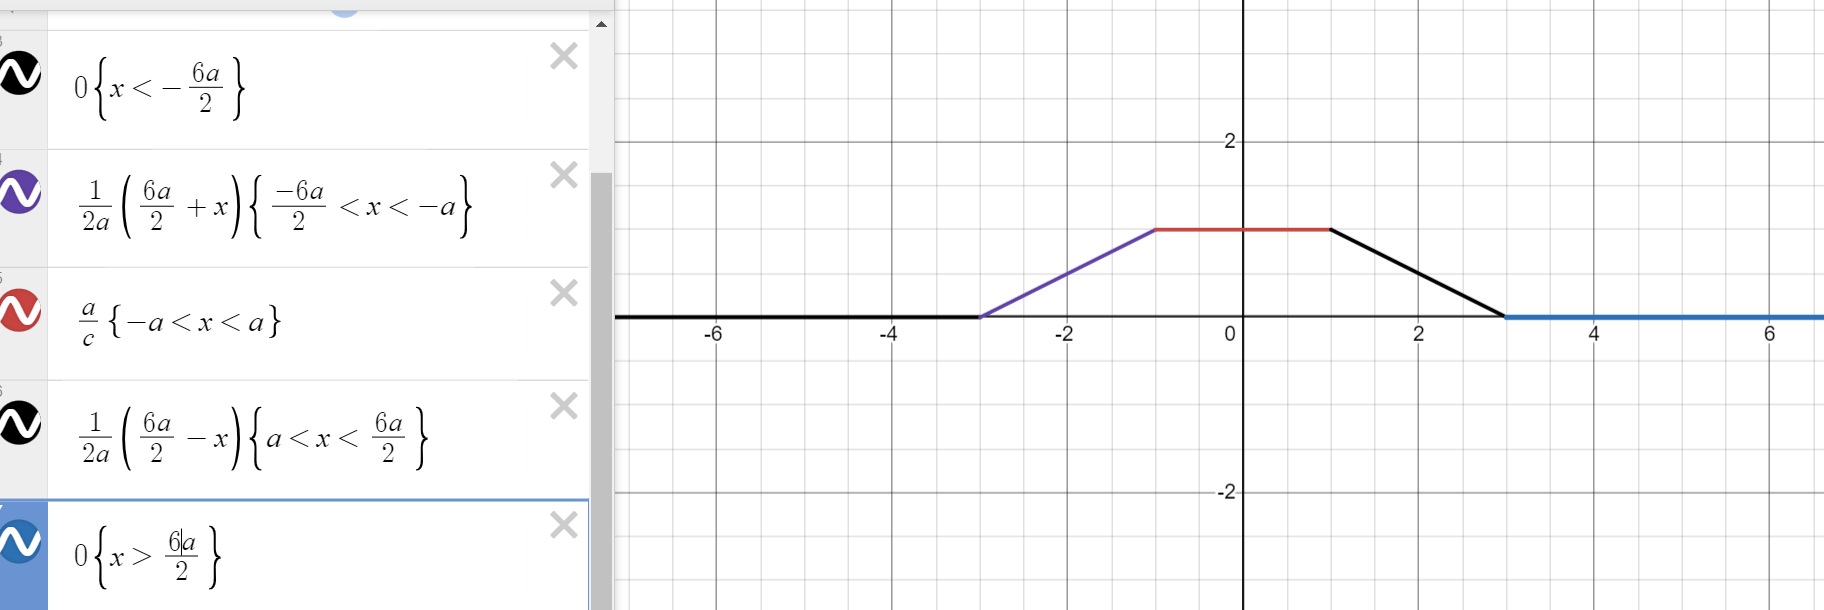
\includegraphics[scale = 0.5]{HW3IMG/14.png}
\end{center}


\textbf{Case 5: $t = 5a/c$}\\
We can see that $x \pm 5a$ becomes the boundary of the interval. \\
We can consider the following cases:
\begin{itemize}
    \item $ x \in (-4a, 4a)$
    \item $ x \in (4a, 6a)$
    \item $ x \in (6a, \infty)$
\end{itemize}
\textbf{Subcase 1: $x \in (-4a, 4a)$}\\
$$(x-5a, x+5a) \cap (-a,a) = (-a,a)$$
$$u(x,5a/c) = \frac{1}{2c} \int_{-a}^{a} ds = \frac{a}{c}$$

\textbf{Subcase 2: $x \in (4a, 6a)$}\\
$$(x-5a, x+5a) \cap (-a,a) = (x-5a, a)$$
$$u(x,5a/c) = \frac{1}{2c} \int_{x-5a}^{a} ds = \frac{1}{2c}({6a}-x)$$

\textbf{Subcase 3: $x \in (6a, \infty)$}\\
$$(x-5a, x+5a) \cap (-a,a) = \emptyset$$
$$u(x,5a/c) = \frac{1}{2c} \int_{a}^{a} ds = 0$$

\textbf{Plotting the graph}\\

\begin{center}
    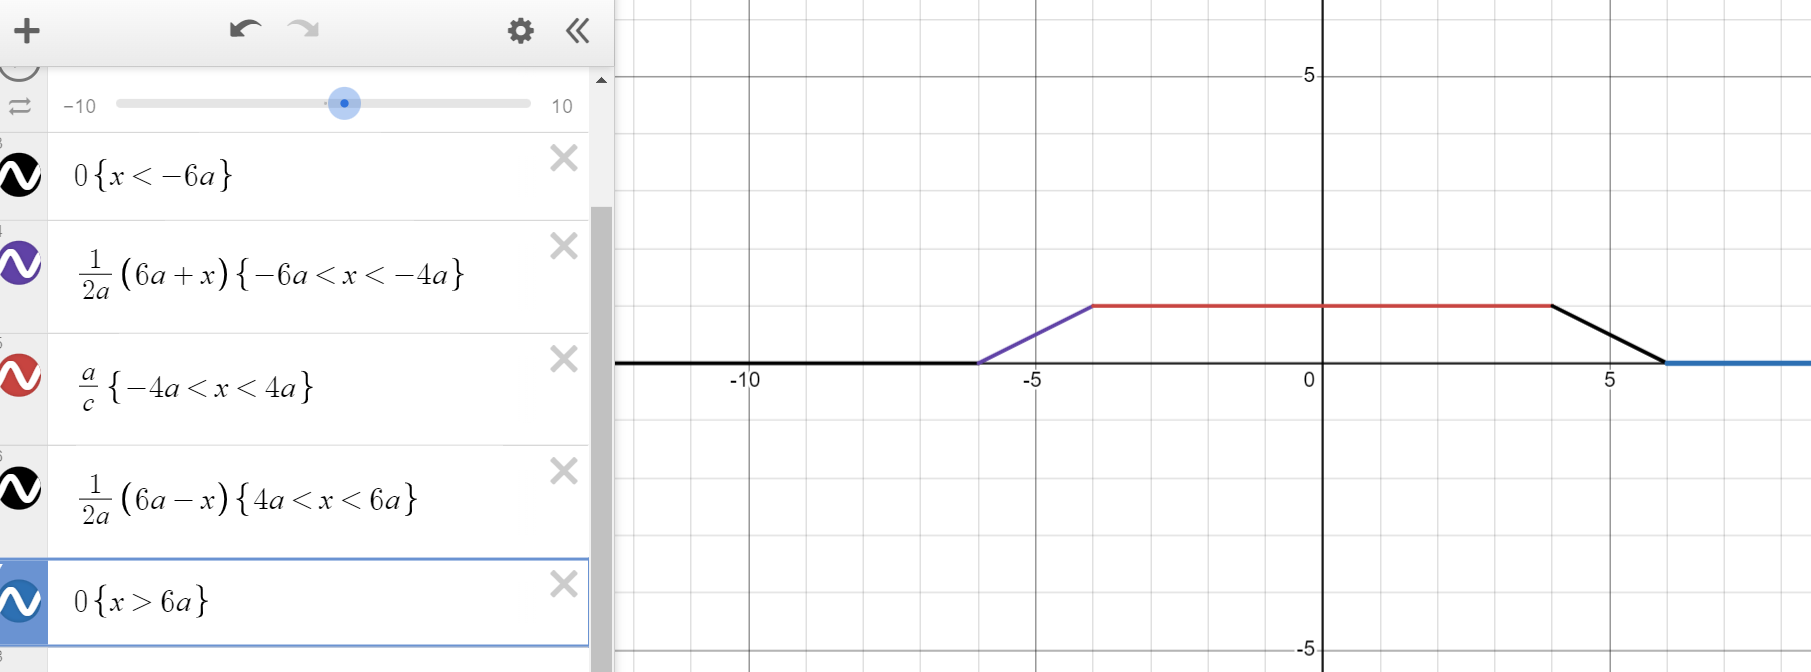
\includegraphics[scale = 0.5]{HW3IMG/15.png}
\end{center}

\question Section 2.1 Problem 9
Solve $u_{xx} -3u_{xt} -4u_{tt} = 0$ for $u(x,0) = x^2$ and $u_t(x,0) = e^t$.\\
\textbf{Solution:}\\
To solve this we can use the factorization method. We can write the equation as:
$$ \left( \frac{\partial}{\partial x} - 4 \frac{\partial}{\partial t} \right) \left( \frac{\partial}{\partial x} + \frac{\partial}{\partial t} \right) u = 0$$
Let $v = \frac{\partial}{\partial x} + \frac{\partial}{\partial t}$. We can write the equation as:
$$ \left( \frac{\partial}{\partial x} - 4 \frac{\partial}{\partial t} \right) v = 0$$
We now have a system of first second order odes:
$$
\begin{cases}
    \frac{\partial u }{\partial t} + \frac{\partial u}{\partial x} = v \\
    -\frac{1}{4}\frac{\partial v}{\partial x} + \frac{\partial v}{\partial t} = 0
\end{cases}
$$

We can see that alond the curves of the tx plane:
$$ \frac{dx}{dt} = -\frac{1}{4}$$
Thus we can rewrite the solution $v$ as a function of $x + \frac{1}{4}t$ and $x(\xi, 0) = \xi$ as we know this is the solution on this characteristic curve.\\
We can also plug this back into the first equation to get:
$$ \frac{\partial u}{\partial t} + \frac{\partial u}{\partial x} = v = f(x + \frac{1}{4}t)$$
We can now solve this equation using the method of characteristics. We have:
$$ \frac{dx}{dt} = 1$$
Thus $x(\eta, 0) = \eta$ Thus the equation becomes:
$$ \frac{du}{dt} = f(x+\frac{1}{4}t)$$
We also know that $\eta = x -t$ Thus:
$$ \frac{du}{dt} = f(\eta + \frac{5}{4}t)$$
Integraring both sides get
$$ u = \int f(\eta + \frac{5}{4}t) dt + g(\eta)$$
For arbitray functions $f$ and $g$. 
Now converting back to the original variables we get:
$$ u(x,t) = \int f(x + \frac{1}{4}t) dt + g(x-t)$$
We can now use the initial conditions to solve for $f$ and $g$. We have:
$$ u(x,0) = x^2 = f(x) dt + g(x)$$
$$ u_t(x,0) = e^t = \frac{1}{4}f'(x) + g'(x)$$
We can now solve for $f$ and $g$ to get the solution.\\
\textbf{Solving for $f$ and $g$}\\
We can see that $f' +g' = 2x$ and $\frac{1}{4}f' + g' = e^t$\\
We can see that $f'  = \frac{8}{5}x + \frac{4}{5}e^t$ and $g' = \frac{2}{5}x - \frac{4}{5}e^t$\\
Thus
$$ f = \frac{4}{5}x^2 + \frac{4}{5}e^t $$
$$ g = \frac{1}{5}x^2 - \frac{4}{5}e^t $$
Now pluggin back in the $x + \frac{1}{4}t$ and $x -t$ we get:
$$u(x,t) = x^2 +\frac{1}{4}x^2 + \frac{4}{5}e^{x-t}(e^{5t/4}-1)$$

\question Section 2.2 Problem 2
for a solution $u(x,t)$ of the wave equation with $\rho = T = C = 1$, the enrgy density is defined as $e = \frac{1}{2}(u_t^2 + u_x^2)$ and the momentum density as $p = u_t u_x$. \\
a) Show that $\frac{\partial e}{\partial t} = \frac{\partial p}{\partial x}$ and $\frac{\partial p}{\partial t} = \frac{\partial e}{\partial x}$\\
b) Show that both $e(x,t)$ and $p(x,t)$ satisfy the wave equation.\\
\textbf{Solution:}\\
\textbf{a}:\\
Since we know that u solves the wave equation we have that:
$$ u_{tt} = u_{xx}$$
We can now calculate the partial derivatives of $e$ and $p$:
$$ \frac{\partial e}{\partial t} = u_t u_{tt} + u_x u_{xt}$$
$$ \frac{\partial p}{\partial x} = u_{tx} u_x + u_t u_{xx}$$
We can sub $u_{tt} = u_{xx}$ to get:
$$ \frac{\partial e}{\partial t} = u_t u_{xx} + u_x u_{xt} = u_t u_{xx} + u_x u_{tx} = u_t u_{xx} + u_x u_{tt} = u_t u_{xx} + u_x u_{xx} = (u_t u_x)_x = \frac{\partial p}{\partial x}$$
Similarly we can calculate the other partial derivative:
$$ \frac{\partial p}{\partial t} = u_{tt} u_x + u_t u_{xt} = u_{xx} u_x + u_t u_{xt} = u_{xx} u_x + u_{tx} u_t = u_{xx} u_x + u_{xt} u_t = (u_x u_t)_x = \frac{\partial e}{\partial x}$$

\textbf{b}:\\
Since we know from part a that
$$\begin{cases}
    p_t = e_x \\
    e_t = p_x
\end{cases}$$
We can take the t and x derivative of both sides for the top and bottom respectively
$$\begin{cases}
    p_{tt} = e_{xt} \\
    e_{tx} = p_{xx}
\end{cases}$$
Clearly $p$ solves the  wave equation.\\
Now if we switch the derivative to take the x and t derivatives for top and bottom respectively we get:
$$\begin{cases}
    p_{xt} = e_{xx} \\
    e_{tt} = p_{tx}
\end{cases}$$
Thus $e$ also solves the wave equation.

\question Section 2.2 Problem 5
For a damped string, equation (1.3.3), show that the energy decreases.\\
The equation is defined by $u_{tt} - c^2 u_{xx} + ru_t = 0$\\
\textbf{Solution:}\\
We need to show that the t derivative of the $KE +PE$ is negative.\\
We have that the $KE = \frac{1}{2}u_t^2 = \frac{1}{2}\rho \int_R u_t^2 dx$
$$ KE_t = \frac{1}{2}\rho \int_R 2u_t u_{tt} dx $$
Upon subbing in the wave equation we get:
$$ KE_t = \rho \int_R u_t (c^2 u_{xx} - ru_t) dx = \rho c^2 \int_R u_t u_{xx} dx - \rho r \int_R u_t^2 dx$$
Once we integrate by parts and consider that $c^2 = T/\rho$ we get 
$$ KE_t = T(u_tu_x)|_R - T\int_R u_{tx}u_x dx - \rho r \int_R u_t^2 dx$$
$$ KE_t = -\frac{1}{2}T \frac{d}{dt} \int_R u_x^2 dx - \rho r \int_R u_t^2 dx$$
Potential energy is defined as
$$ PE = \frac{1}{2} T \int_R u_x^2 dx $$
Thus the time derivative total energy is:
$$ KE_t + PE_t = -\rho r \int_R u_t^2 dx < 0$$
Thus the energy decreases.

\question Section 2.3 Problem 4
Consider the diffusion equation $u_t = u_{xx}$ in $x \in (0,1)$ and $t \in (0, \infty)$ with $u(0,t) = u(1,t) = 0$ and $u(x,0) = 4x(1-x)$.\\
a) Show that $0 <u(x,t) < 1$ for all $x \in (0,1)$ and $t > 0$.\\
b) Show that $u(x,t) = u(1-x,t)$ for all $x \in (0,1)$ and $t > 0$.\\
c) Use the energy method to show that $\int_0^1 u^2 dt$ is a strictly decreasing function of $t$.\\
\textbf{Solution:}\\
\textbf{a:}\\
We can utilize the minimum and maximum principles\\
For the bottom bound we can use the minimum principle and see that on the $\Gamma$ boundary we have $u(0,t) = u(1,t) = 0$ and $u(x,0) = 4x(1-x)$ which is clearly positive. Thus the minimum value of $u(x,t)$ is 0.\\
For the upper bound we can use the maximum principle and see that the maximum value on the boundary is at $x = \frac{1}{2}$ and $t = 0$ which is 1. Thus the maximum value of $u(x,t)$ is 1.\\
Thus $0 < u(x,t) < 1$ for all $x \in (0,1)$ and $t > 0$.\\
\textbf{b:}\\
We can clearly see that $u(1-x,t)$ solves the diffusion equation as 
$$ \frac{\partial}{\partial t}u(1-x,t) = u_t$$
$$ \frac{\partial}{\partial x} u(1-x,t) = -u_x$$
$$ \frac{\partial^2}{\partial x^2} u(1-x,t) = u_{xx}$$
Since $u_t = u_{xx}$ we have that $u(1-x,t)$ solves the diffusion equation.\\
Additionally \\
The range of $u(x,t)$ is $(0,1)$ and the range of $u(1-x,t)$ is also $(0,1)$\\
Additionally 
$$ u(0,t) = u(1,t) = 0 \implies u(1,t) = u(0,t) = 0$$
As well as 
$$u(x,0) = 4x(1-x) \implies u(1-x,0) = 4(1-x)x $$
\textbf{c:}\\
We can first consider the diffusion equation in the form of $u_t = u_{xx}$\\
Then we can multiply by $u$ on both sides to get $u u_t = u u_{xx}$\\
We can rewrite to get $\frac{1}{2} \frac{\partial}{\partial t} u^2 = (u_x u )_x - u_x^2$\\
Now integraring over the interval $(0,1)$ we get:
$$ \frac{1}{2} \int_0^1 \frac{\partial}{\partial t} u^2 dx = \int_0^1 (u_x u )_x dx - \int_0^1 u_x^2 dx$$
$$ \frac{1}{2} \frac{d}{dt} \int_0^1 u^2 dx = (u_x u )|_0^1 - \int_0^1 u_x^2 dx$$
$$\frac{d}{dt} \int_0^1 u^2 dx = - 2\int_0^1 u_x^2 dx$$
Clearly since the RHS is always negative, the LHS is always negative. Thus the integral is a strictly decreasing function of $t$.

\question Section 2.3 Problem 6
Prove the comparison principle for the diffusion equation: If u and v are two
solutions, and if $u \leq v$ for $t = 0$, for $x = 0$, and for $x = l$, then $u \leq v$ for $0 \leq t <\infty, 0 \leq  x\leq  l$.
\textbf{Solution:}\\
Since we know that $u$ and $v$ are solutions to the diffusion equation we have that $u_t = u_{xx}$ and $v_t = v_{xx}$\\
Also we can consider the function $w = u - v$\\
Since we know that $u \leq v$ for $t = 0$, for $x = 0$, and for $x = l$, we have that $w \leq 0$ for $t = 0$, for $x = 0$, and for $x = l$\\
We can also consider that $w_t = u_t - v_t = u_{xx} - v_{xx} = w_{xx}$\\
The middle terms of the equation can factor to get: $(u-v)_t = (u-v)_{xx}$\\
Since clearly $w$ solves the diffusion equation and $w \leq 0$ for $t = 0$, for $x = 0$, and for $x = l$, we have that $w \leq 0$ for $0 \leq t <\infty, 0 \leq  x\leq  l$\\
Thus we can say tat $u \leq v$ for $0 \leq t <\infty, 0 \leq  x\leq  l$ due to the minimum principle of $u - v$

\question Section 2.3 Problem 8
Consider the diffusion equation on $(0,l)$ with the Robin BC $u_x(0,t) - a_0 u(0,t) = 0$ and $u_x(l,t)+a_lu(l,t) = 0$ If $a_0 > 0$ and $a_l > 0$, use the energy method to show that the endpoints contribute to the decrease of $\int_0^l u^2 dx$\\
\textbf{Solution:}\\
The boundary conditions are: 
$$u_x(0,t) - a_0 u(0,t) = 0 \to u_x(0,t) = a_0 u(0,t)$$
$$u_x(l,t) + a_l u(l,t) = 0 \to u_x(l,t) = -a_l u(l,t)$$
We can then consider the diffusion equation: $u_t = ku_{xx}$\\ 
We can multiply by $u$ on both sides to get $u u_t = ku u_{xx}$\\
We can rewrite to get $\frac{1}{2} \frac{\partial}{\partial t} u^2 = (u_x u )_x - u_x^2$\\
Then integrating over the interval $(0,l)$ we get:
$$ \frac{1}{2} \int_0^l \frac{\partial}{\partial t} u^2 dx = k\int_0^l (u_x u )_x dx - k\int_0^l u_x^2 dx$$
$$ \frac{1}{2} \frac{d}{dt} \int_0^l u^2 dx = k(u_x u )|_0^l - k\int_0^l u_x^2 dx$$
$$\frac{1}{2} \frac{d}{dt} \int_0^l u^2 dx = k[u_x(l,t)u(l,t) - u_x(0,t)u(0,t)] - k\int_0^l u_x^2 dx$$
$$\frac{d}{dt} \int_0^l u^2 dx = 2k[-a_l u^2(l,t) - a_0 u^2(0,t)] - 2k\int_0^l u_x^2 dx$$
Since $a_0 > 0$ and $a_l > 0$ the lhs is all negative. Thus the endpoints contribute to the decrease of $\int_0^l u^2 dx$


\end{questions}
\end{document}